% !TeX root = ../DistributedConsensus.tex
% !TeX spellcheck = en_GB
\chapter{Reducing Histories to Orders of Execution}\label{chap:order-of-execution}
	In this chapter, it is examined how it is possible to find an order of execution from a valid global history and it is shown that consensus can be reached on the found order of execution with an election.

\section{Order of Execution}
	A valid global history represents every action that has occurred on all the events of the workflow.
	It is desired to find an order of execution with excess information in the history removed without losing information regarding the order of the executions. To do this, we need to represent an execution as a single entity and furthermore find the minimum equivalent graph of the resulting order.
	
	\subsection{Single Entity Representing an Execution}
	In order to find a single representation of an execution, one approach could be to examine if a single action of an execution could describe all the relations to all the other executions. Doing this involves filtering all actions not chosen to be the representative of the execution, and since filtering nodes also removes their edges, happen before relations between executions would be lost. Therefore it is necessary to add a direct edge between representatives if there is already a path from one to the other in the history. Since the history is represented as a directed acyclic graph, the transitive closure of the graph provides the desired relations. Having found the transitive closure of the history, actions that are not the representative for an execution are removed from the graph along with their edge.
	
	Since every execution has actions of types \textit{Execute start} and \textit{Execute finish}, choosing one of these as the representative seems like a sensible choice. For any execution in a history, an action of type \textit{Execute start} always has a path to an action of type \textit{Execute finish}. Therefore the transitive property of directed acyclic graphs, states that in an execution the reachability of an action of type \textit{Execute start} is a superset of the reachability of the action of type \textit{Execute finish}, and therefore it contains more information about happens before relations. To conclude, actions of type \textit{Execute start} are the most sensible choice of these two types.
	
	A situation where actions of type \textit{Execute start} is chosen as representatives is shown in \autoref{fig:problem:trans}. What becomes apparent in this figure, is that the first execution of event $A$ must happen before the first execution of event $B$. This is because two events that have a happen before relation must have any kind of relation in the workflow. If the events have a relation in the workflow, then they must execute serially equivalent. This ensures that an execution of one of the events must happen either before, or after an execution of the other. Therefore another approach must be taken.
	
	\newpar In \cite{sedgewick2011algorithms}, Sedgewick et. al. describes an implementation of transitive closure, which has a time complexity of $\mathcal{O}(V * (V + E))$ where V is the number of nodes and E is the number of edges in the graph.
	
	\begin{figure}
		\centering
		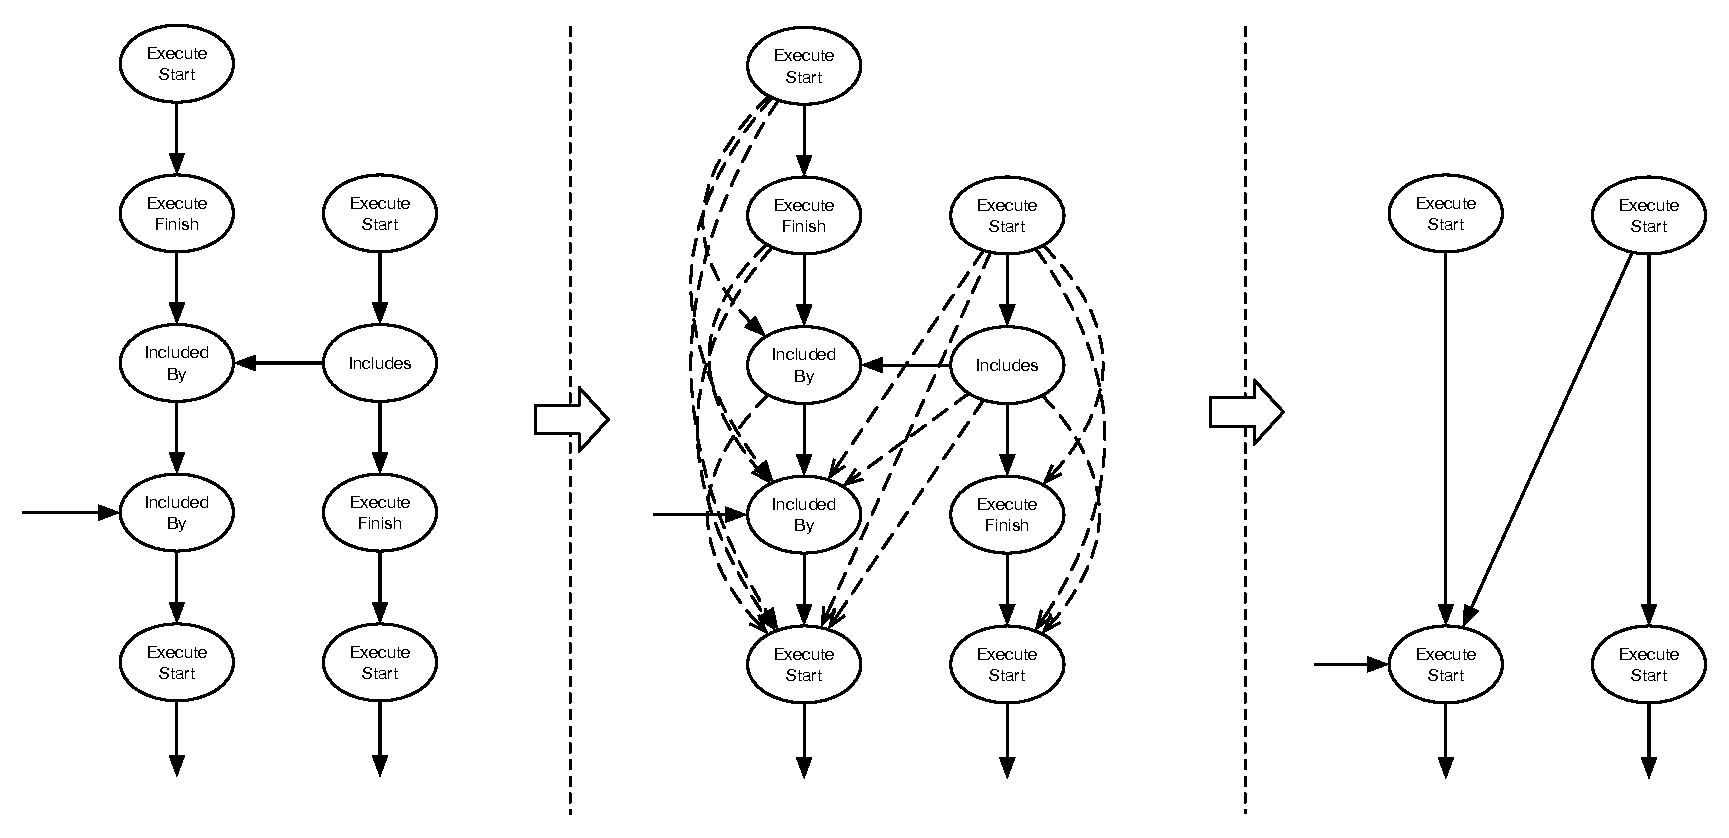
\includegraphics[width=\textwidth]{5orderofexecution/images/trans.pdf}
		\caption{The result of finding the transitive closure on from the actions of an event. Note that the topmost executions happen concurrently. So do the two lower executions.}
		\label{fig:problem:trans}
	\end{figure}
	
	\subsection{Collapsing}
	As described above, transitive closures are not an ideal way of representing an execution as a single entity and therefore collapsing is introduced.
	
	\newpar In \autoref{def:execution} an execution is defined to be all the actions representing the effects of the execution, as well as two actions with types \textit{Execute start} and \textit{Execute finish}. Even though incoming actions are stored on other events than the ones performing the executions, these actions are still initiated by the executing event and are therefore seen as being part of the execution. Since an event is only affected by the effects of other events or itself executing, any action is always part of \textit{some} execution of \textit{some} event, and therefore no action can happen outside an execution.
	
	\newpar In \autoref{inv:historyinvariant} it is said that if a single action in one execution happens before another action in another execution, then no action from the second execution can happen before an action in the first. In other words this means, if there exists an action in execution $A$, that happens before an action in execution $B$, then $A$ happens before $B$, and $B$ cannot happen before $A$. Note that this does not mean that all actions in $A$ happens before all actions in $B$, which means some of the actions are in fact concurrent. This creates the need for an argument that $A$ \textit{does} happen before $B$ despite that some actions are concurrent.
	
	\newpar As stated in the previous section, because of serial equivalence, two events, where one has a relation to the other, can only execute in a way such that the result is the same as if one had executed before the other. Therefore any happens before relation any action in an execution has with any action outside of that execution actually applies to all actions in the execution. When this is the case, every action inside an execution is equal in terms of happens-before relations and therefore we can \textit{collapse} the execution into one single entity.
	
	\newpar An example of collapsing actions into executions are shown in \autoref{fig:orderofexecution:collapse}. This is the same example as used when describing transitive reduction. We now see that the first execution of $A$ happens before the first execution of $B$.
	
	\begin{figure}[H]
		\centering
		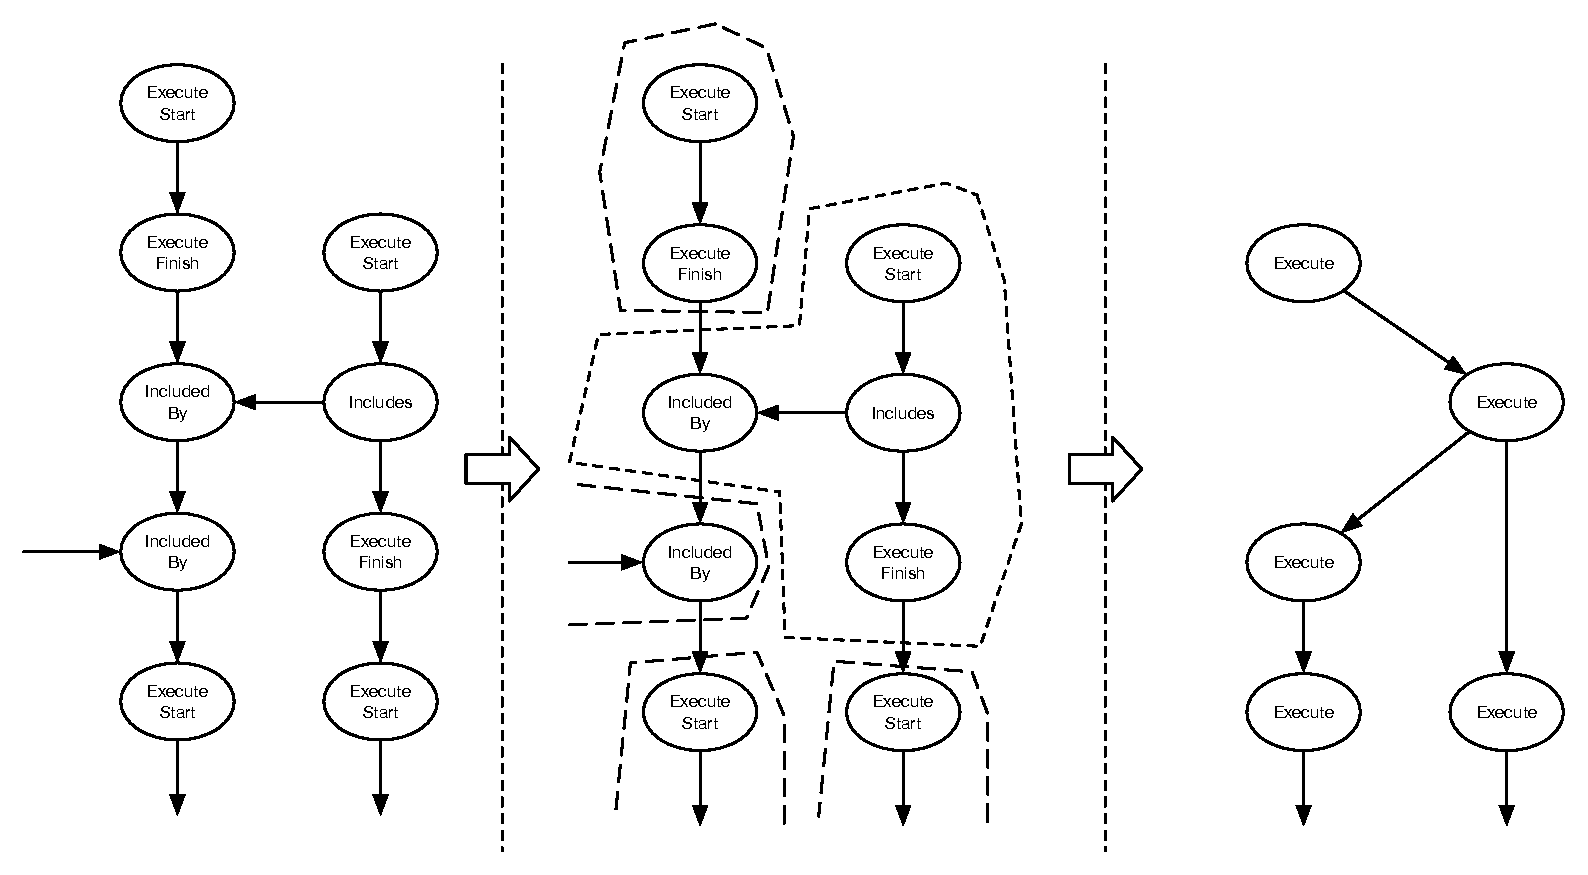
\includegraphics[width=\textwidth]{5orderofexecution/images/collapse.pdf}
		\caption{The result of finding an execution using \textit{Collapse}. Note that executions that previously were concurrent (\autoref{fig:problem:trans}) are now ordered.}
		\label{fig:orderofexecution:collapse}
	\end{figure}
	
%	\newpar It then is necessary to research a way to \textit{collapse} an execution in order to overcome these problems. \textit{Collapsing} constitutes looking at all actions between an \texttt{ExecuteStart} action and an \texttt{ExecuteFinish} action of an event and connecting these events into a single entity, representing an entire execution. 


%	\newpar When actions contained in an execution have been found, it is necessary to decide what should happen to the grouping of the actions. It is desired to keep all relations intact, to avoid modifying the history and only simplify it. 
	
%	By pointing all ingoing edges to the current event towards a new \textit{collapsed node}, and adding all outgoing edges to the new node, this is accomplished. This new \textit{collapsed node} then represents the entire execution. 

%	In the implemented solution the the \texttt{ExecuteFinish} type has been chosen to denote a collapsed execution in order to avoid creating a new action type. As it can be seen in \autoref{fig:after-collapsing} the collapsing of executions results in an order of execution.

	
	\newpar The collapsing algorithm can be be seen in \autoref{alg:collapse}. The algorithm gathers all actions of an execution and, after the single entity execution is created, creates all happens-before relations. 
	
	\noindent One of the properties the collapsed order of execution has, is that, for two executions to be concurrent the executing events must be independent, as described in \cite{debois2015concurrency}, however, not all independent events create concurrent executions. To show that all non-independ events cannot be concurrent, we will show that if any of the properties of independent events are not present between a pair of events, making them non-independent, then collapse will order the executions.
	
	\begin{enumerate}
		\item \textit{No event included by $E$ is excluded by $F$ and vice versa}: This property is violated if $E$ includes an event, $G$ that $F$ excludes. The incoming actions on $G$ will allow collapse to order the executions of $E$ and $F$.
		\item \textit{$E$ requires a response from some $G$ iff $F$ does}: This property is violated if $E$ has a response relation to $F$, but $F$ does not have a response relation to itself. In this case, an execution of $E$ results in incoming actions on $F$. Any execution of $F$ is always before or after these incoming actions.
		\item \textit{Neither event is a condition for the other}: This property is violated if $E$ is a condition for $F$. In this case the incoming actions from the execution of $F$ on $E$, enables the ordering of executions of the events.
		\item \textit{Neither event includes or excludes the other}: This property is violated if $E$ includes $F$. In this case the incoming actions from the execution of $E$ on $F$, enables the ordering of executions of the events.
		\item \textit{Neither event includes or excludes a condition of the other}: This property is violated if $E$ excludes $G$ which is a condition of $F$. Recall that conditions in the implementation are checked by the executing event. This means that any execution of $F$ will result in incoming actions on $G$. Also the execution of $E$ will result in incoming actions on $G$. Therefore the incoming actions on $G$ will allow collapse to order the executions of $E$ and $F$.
	\end{enumerate}
	
	To argue that the collapse algorithm correctly describes the relations between executions \autoref{inv:historyinvariant} is examined. It states that if there exist any action in execution $A$ with a relation to execution $B$, then it must not be true the other way around. Therefore for collapse to be correct each single execution entity must have the same property. 
	
	Since the set of relations the single entity has to other executions is the union of the set of all the actions had to other executions, it must be so that the set cannot contain relations which violates the invariant, because then the invariant would already be broken before the collapse. 
	
	By proof of contraditction, it it was so that the invariant is broken in the union set, then there is a value where $A$ happens before $B$ and $B$ happens before $A$, then the original collection of sets must already have had these two relations.
	
	\todo[inline]{Check if you like this argumentation.}
	
	\begin{algorithm}[H]
		\begin{algorithmic}
			\Function{Collapse}{graph}\State
				locals: CollapseMap: Mapping from old to newaction IDs.
				\State\hspace{28pt} Result: Graph, initially empty
				\State
				\State ExecuteStarts $\leftarrow$ \Call{Filter}{type = ExecuteStart, graph} \State
				Executions $\leftarrow$ \Call{Map.map}{FindSingleExecution, ExecuteStarts}
				\ForAll{executions in Executions}\State
					CollapseMap $\leftarrow$ \Call{CreateExecutionMap}{execution, newExecutionId, CollapseMap}
				\EndFor
				\ForAll{oldActionID, newActionID in CollapseMap}
					\State
					NewAction $\leftarrow$ Action with \State\hspace{28pt}ID = newActionID and \State\hspace{28pt}Edges = edges from oldActionID in graph mapped to new IDs\State
					Result $\leftarrow$ \Call{AddNode}{NewAction, Result} \State\Comment{This requires AddNode to merge edge sets when existing nodes are added}
				\EndFor
				
			\EndFunction
			\State
			\Function{FindSingleExecution}{startAction}
				\State locals: execution
				\While{startAction.Type $\neq$ ExecuteFinish} \State
					execution $\leftarrow$ \Call{AddRange}{startAction.Edges, execution}
				\EndWhile\State
				\Return execution
			\EndFunction
			\State
			\Function{CreateExecutionMap}{ActionSet, newActionId, accumulatorMap}
				\ForAll{actions in ActionSet}\State
					accumulatorMap $\leftarrow$ \Call{Add}{action.Id, newActionId, accumulatorMap}
				\EndFor \State
				\Return accumulatorMap
			\EndFunction
		\end{algorithmic}
		\caption{Collapse algorithm}
		\label{alg:collapse}
	\end{algorithm}\todo[inline]{Mikael: Jeg kunne godt tænke mig hvis vi definerede hjælperne i teksten, og kun havde essensen af collapse tilbage. Jeg ved ikke om dette er en \textbf{for} grov frasortering?}
	\todo[inline]{Fisk: Synes det lyder som en god idé.}
	
	\newpar The algorithm runs in a time complexity of $O(n^2)$ where $n$ is the number of actions in the history. This must be so since $CreateExecution$ runs linearly in $n$ if $Add$ on $map$ is constant and $CreateExecution$ worst case gets called $n/2$ times if every action in the history are executions. \todo{write better more correct yes}
	
	\subsection{Transitive Reduction}
	\begin{figure}[H]
		\centering
		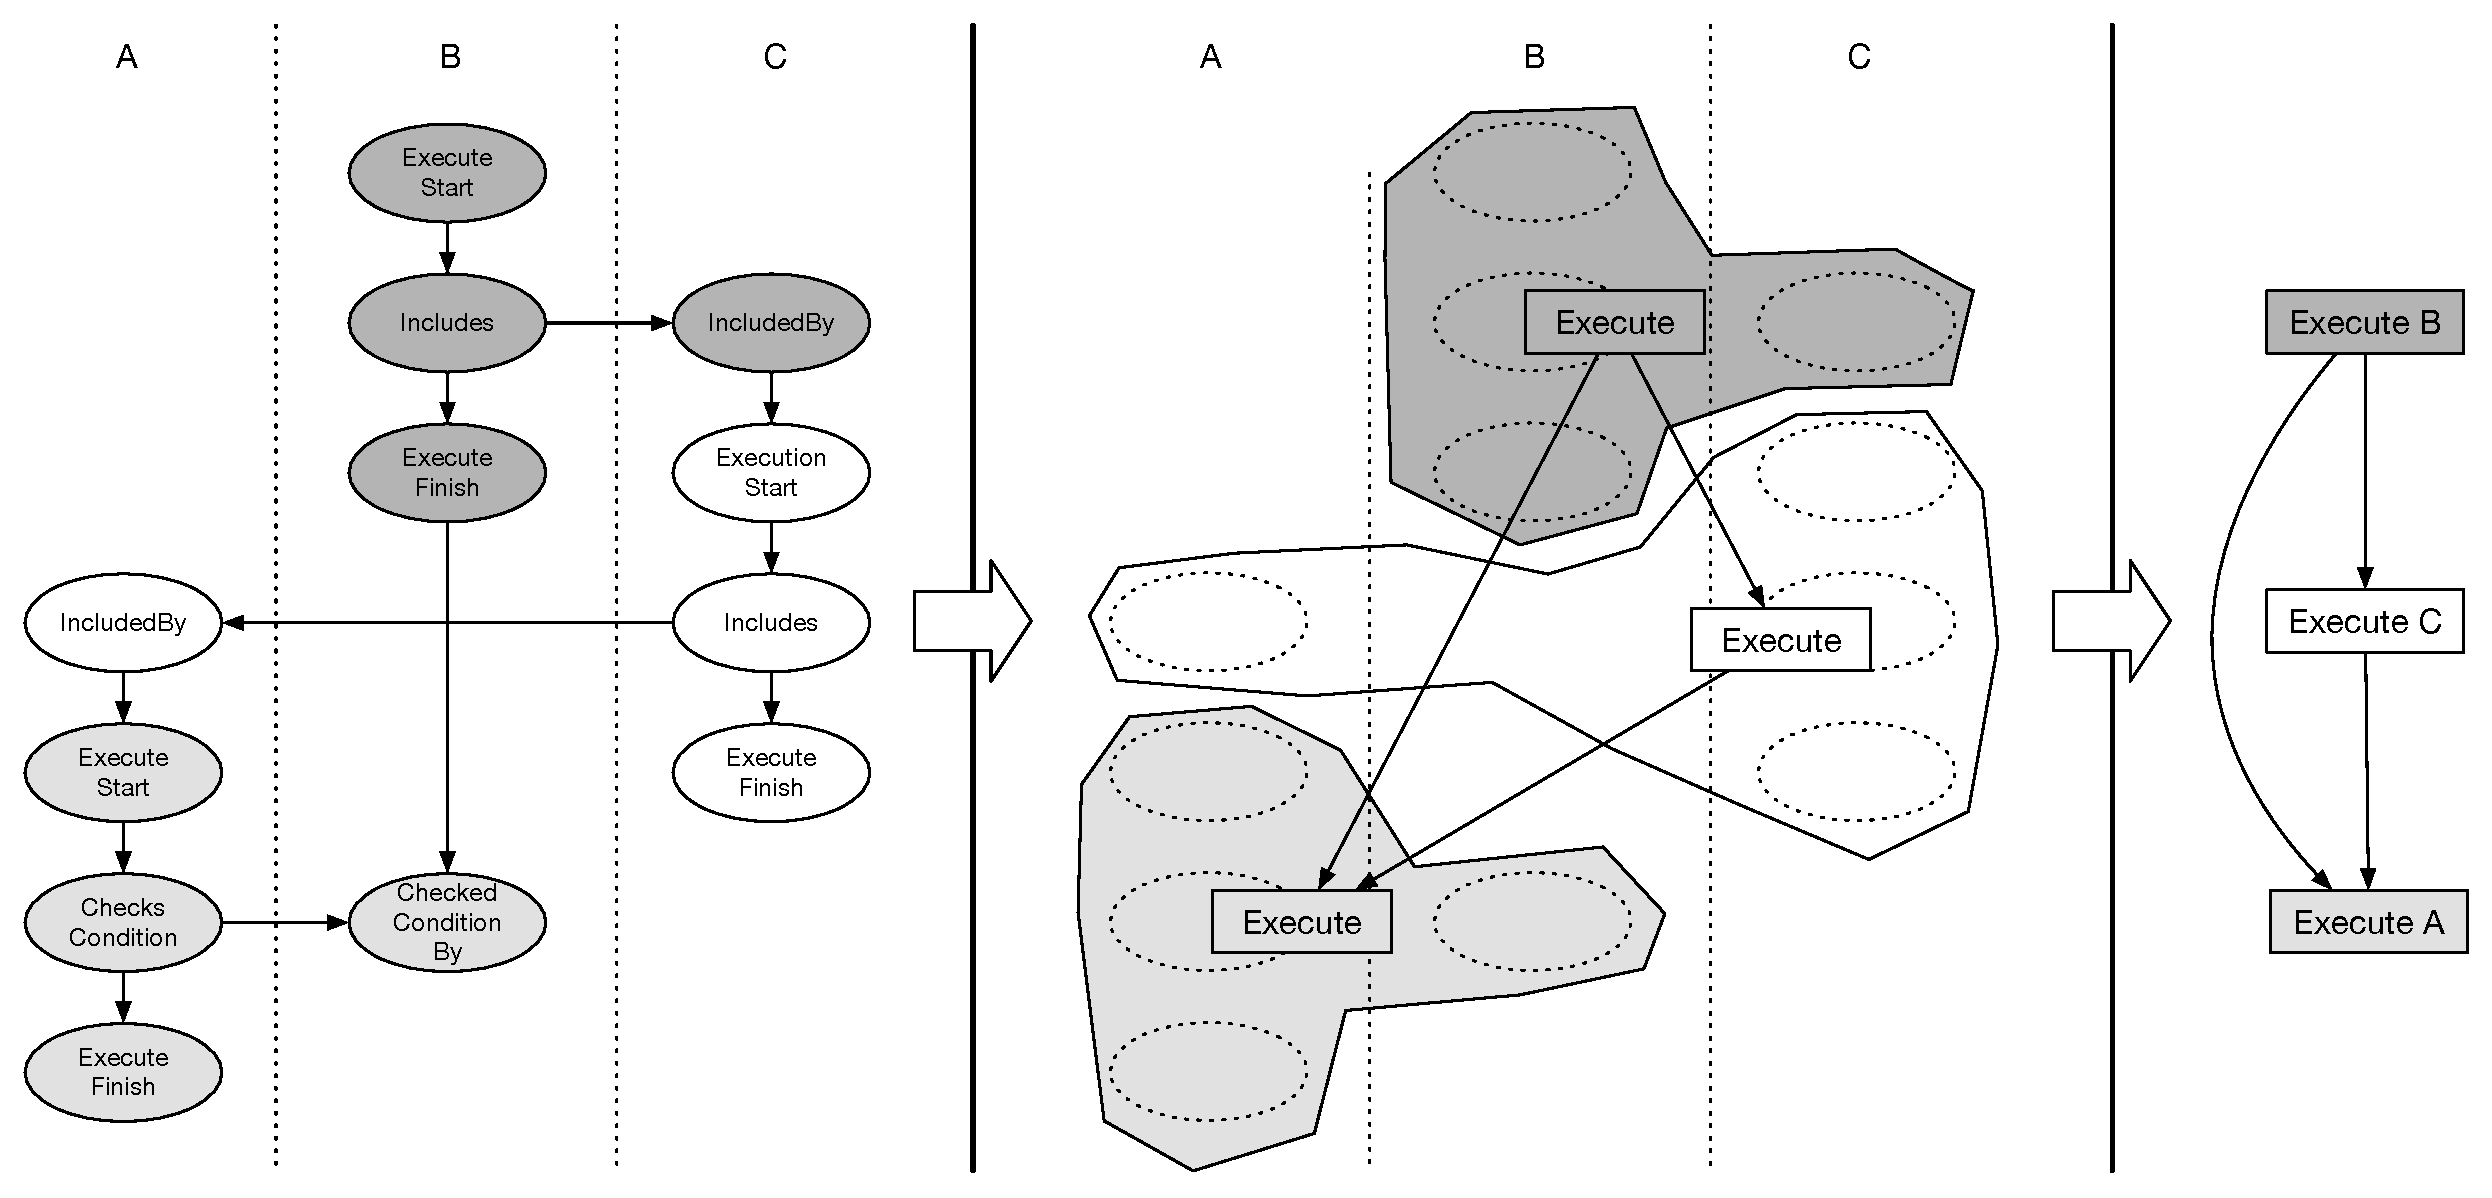
\includegraphics[width=\textwidth]{5orderofexecution/images/transitive-example-collapse.pdf}
		\caption{The result of collapsing actions in the histories of three events.}
		\label{fig:orderofexecution:collapsing}
	\end{figure}
	
	\newpar Redundant edges might still exist in the history after executions of the history have been collapsed, as seen in \autoref{fig:orderofexecution:collapsing}. An edge is redundant in cases where there exists a non-direct path from an execution to another execution, but there also exists a direct edge between the two executions. In this case the direct edge is redundant and can be removed, since it does not contribute extra information in regards to the ordering of the executions as it only explicitly expresses what is implicitly available. Removing it will not affect the ordering or reachability of the order of execution, but rather simplify the order of execution.
	
	\newpar An example of a redundant edge in a collapsed order of execution can be seen in figure \autoref{fig:orderofexecution:collapsing}. The figure illustrates a case where a redundant edge exists between event $A$ and event $B$, since the edge from event $B$ through $C$ provides more information about the order in which the executions occurred. 
	Recall that the order of execution is represented as a directed acyclic graph and that it is possible to find a minimal equivalent graph for such a graph. 
	
	\newpar In directed acyclic graphs the transitive reduction of a given graph is a graph with the fewest possible number of edges, but the same reachability as the given graph.	That is, if there exists a path from an edge $x$ to an edge $y$ in graph G, there must also be a path from $x$ to $y$ in the transitive reduction of $G$, and vice versa.
		
	Furthermore, the transitive reduction will always be a subgraph of the given graph. For that reason the transitive reduction corresponds to the minimum equivalent graph.\todo[inline]{Jeg (Mikael) har det lidt med subgraph som jeg har det med subset. Jeg er ikke helt sikker på hvad det betyder i denne sammenhæng - Altså, jeg synes ikke det hjælper til min forståelse af problemet (hvilket jeg i øvrigt synes er udpenslet nok på dette tidspunkt.)}
	
	The implementation for finding the transitive reduction on an order of execution is shown in \autoref{alg:orderofexecution:reduction}.
	
	\begin{algorithm}[H]
		\begin{algorithmic}
			\Function{Transitive-Reduction}{$history$}
				\ForAll{$execution1$ \textbf{in} $history$}
					\ForAll{$execution2$ \textbf{in} $history$}
						\If{\Call{pathExists}{$execution1$, $execution2$, $history$}}
							\ForAll{$execution3$ \textbf{in} $history$}
								\If{\Call{edgeExists}{$execution2$, $execution3$, $history$}}
									\If{\Call{edgeExists}{$execution1$, $execution3$, $history$}}
										\State $history$ $\leftarrow$ \Call{removeEdge} {$execution1$, $execution3$, $history$}
									\EndIf
								\EndIf
							\EndFor
						\EndIf
					\EndFor
				\EndFor
			\State
			\Return $history$
			\EndFunction
		\end{algorithmic}
		\caption{Transitive Reduction Algorithm}
		\label{alg:orderofexecution:reduction}
	\end{algorithm}
	
	\newpar The shown algorithm for transitive reduction has a time complexity of $O(n^3)$ where $n$ is the number of executions, since the algorithm has three nested for-loops over all executions in the history. This is based on the requirements that $pathExist$ runs in linear time and $edgeExist$ is a constant lookup. In actual use cases the graph will not be totally connected and therefore the innermost loop will not be executed for most executions. \todo{check if pathExists runs linearly}
	
	\begin{figure}[H]
		\centering
		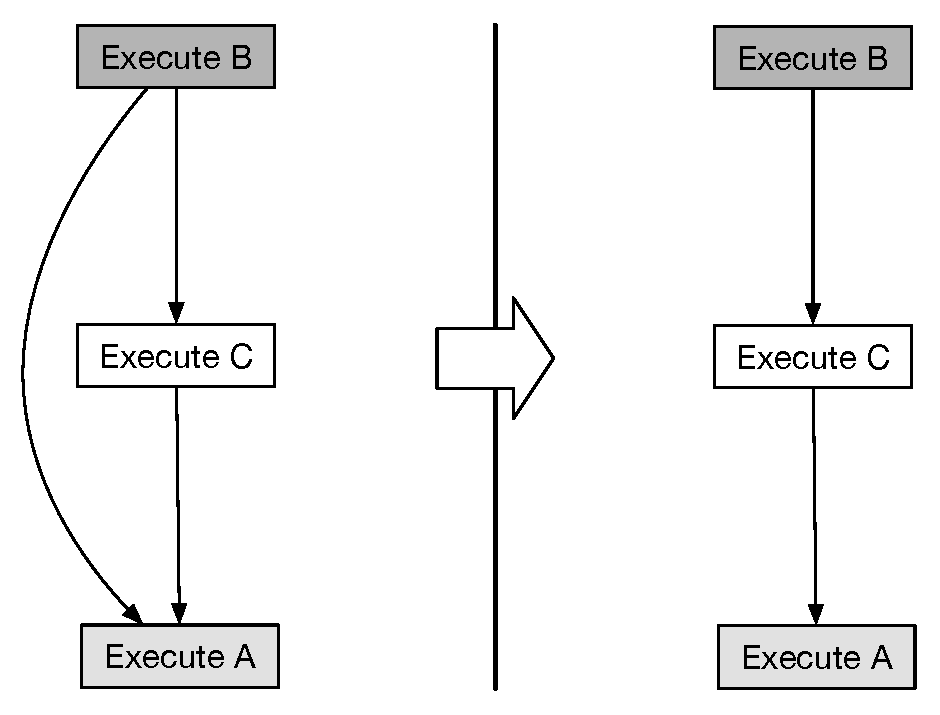
\includegraphics[height=0.35\textheight]{5orderofexecution/images/reduce-before-after.pdf}
		\caption{The result of reducing an order of execution with redundant edges.}
		\label{fig:orderofexecution:reduce-before-after}
	\end{figure}

% Synes ikke det hører til her	
%	\newpar These algorithms do not provide a way to ensure that malicious nodes cannot tamper with the history. As in the case where one event represented the workflow, there is no way of making sure that the event creating the history will not tamper with the history. It would be possible to pinpoint which neighbouring events are malicious if enough of the neighbours have relations to each other. 


	\section{Election} 
	As we have now found an order of execution where (potentially) malicious events have been identified, we want to know if the remaining events can agree upon the rest of order of execution.
	
	\newpar As stated in the problem definition, it is desired to reach consensus on the resulting order of execution, but since no process in the system knows the entire state of a workflow, it is not possible for the events to suggest an order of execution without completing steps alike with the ones described in this report.
	
	\newpar Because we have chosen to let the client know all events in order to retrieve their histories, it is also easy for us to send the resulting order of execution back to them, in order to find out whether or not they can agree to this order.
	
	\newpar When any event receives this order of execution, it can look at its own history and at the received order. The local history can contain executions with outgoing actions between execute start and execute finish actions. Furthermore ingoing relations can be identified as executions of other events from the following rules:
	
	\begin{itemize}
		\item Each counterpart present in actions with ingoing action types must have executed at least once, in order to contact the local event.
		\item If two actions with the same ingoing action type and counterpart are present after each other, this denotes two separate executions of the counterpart event, because each executing event only contacts another event once per relation when executing.
	\end{itemize}
	
	%\newpar Furthermore if an event has sent multiple ingoing requests as part of a single execution, then each of the relations that these actions represent must be present every time that execution has happened.
	%Ovenstående er udkommenteret fordi det relaterer mere til validation end election.
	
	\newpar	Given these rules, the local history can be turned into a "local order of execution".
	\figuretodo{Tilføj figur der viser hvordan en lokal historik kan omdannes til en order of execution der kan bruges til afstemning.}
	
	\newpar Now that the event has created a local order of execution, this order can be used to decide whether or not the event can agree on the global order of execution. If there exists a path from one execution to another in the local order of execution, there must also exist a path between these executions in the global order of execution for the event to agree. Because the local history is totally ordered, the local order of execution must also be totally ordered.\todo[inline]{proof?}
	
	With this property the event can find the local order of execution in the global order. \todo[inline]{The following algorithm assumes that an execution can be found across local and global orders of execution.}Algorithm \ref{alg:vote} outlines how this can be done.
	
	\begin{algorithm}
		\begin{algorithmic}
			\Function{Vote}{localHistory, globalOrderOfExecution}
				\State\hspace{2em}\textbf{returns} \texttt{True} if the paths between executions in the local history are present in the
				\State\hspace{6em}global history. \texttt{False} otherwise.
				\State localOrderOfExecution $\leftarrow$ \Call{MakeLocalOrderOfExecution}{localHistory}
				\State localExecution $\leftarrow$ execution in localHistory with lowest local timestamp
				\While{\Call{IsNotNull}{currentLocalExecution}}
					\If{\Call{IsEmpty}{currentLocalExecution.Edges}}
						\State \Return \texttt{True}
					\EndIf
					\State globalExecution $\leftarrow$ find localExecution in globalOrderOfExecution
					\State nextGlobalExecution $\leftarrow$ find next local execution in globalOrderOfExecution
					\If{\Call{HasPath}{globalExecution, nextGlobalExecution, globalOrderOfExecution}}
						\State\Return \texttt{False}
					\EndIf
					
					\State localExecution $\leftarrow$ \Call{SingleOrNull}{localExecution.Edges}
				\EndWhile
			\EndFunction
		\end{algorithmic}
		\caption{The \textit{\textbf{Vote}} algorithm}
		\label{alg:vote}
	\end{algorithm}
	
	If the history is correct, and the nodes are correct, then the nodes will vote in favour of the history.
	
	It is possible to decide a threshold for the ratio between the number of good nodes and the number of malicious nodes. If the result of the election is better than the threshold, then distributed consensus between the nodes exists for the history. In distributed systems this threshold is normally set to the majority of the participating nodes, which means at least one more than half the amount of nodes.\todo[inline]{Find a source.}
	
	\newpar Election is not an actual vote on the result of the resulting order of execution. Election is instead a confirmation that the algorithm has produced the correct result.
	
	\todo[inline]{Tilføj correctness proof/paragraph. "There should be a theorem or something clearly stating that this algorithm solves the original problem." WIND: i dont know if this was it but i tried PIL NED}
	
	If the algorithm has found the correct solution then correctly functioning events must be decide to accept the result. By proof of contradiction if the correctly functioning events do not vote for the history then that implies that happens before relations are missing from the global history, which would then imply that the proposed global order was incorrect and therefore that the proposer is malicious.
	
	This algorithm solves the initial problem which was to achieve distributed consensus on the order of execution. It does so because each individual event can accept a proposed value by the commander, and if the commander is correct then all the events will have decided the same value, and distributed consensus is hereby achieved.
	
	
	\figuretodo{Tilføj figur: Kan vi på nogen måde vise resultatet af election? FISK: Tror det bliver lidt svært. }